\documentclass{assignment}
\UsingEnglish
\ProjectInfos*{Intro to Communication System}{EE140}{Fall, 2020}{Assignment 11}{Due time : 10:15, Dec 18, 2020 (Friday)}{陈稼霖}{45875852}
\begin{document}
\begin{prob}[8.1, Binary minimum cost detection]
    \begin{itemize}
        \item[(a)] Consider a binary hypothesis testing problem with a priori probabilities $p_0$, $p_1$ and likelihoods $f_{V\vert U}(v\vert i)$, $i=0,1$. Let $C_{ij}$ be the cost of deciding on hypothesis $j$ when $i$ is correct. Conditional on a observation $V=v$, find the expected cost (over $U=0,1$) of making the decision $\tilde{U}=j$ for $j=0,1$. Show that the decision of minimum expected cost is given by
        \[
            \tilde{U}_{\text{mincost}}=\arg\min_j\left[C_{0j}p_{U\vert V}(0\vert v)+C_{1j}p_{U\vert V}(1\vert v)\right]
        \]
        \item[(b)] Show that the min cost decision above can be expressed as the following threshold test:
        \[
            \Lambda(v)=\frac{f_{V\vert U}(v\vert 0)}{f_{V\vert U}(v,1)}\overset{\tilde{U}=0}{\underset{\tilde{U}=1}{\gtreqless}}\frac{p_1(C_{10}-C_{11})}{p_0(C_{01}-C_{00})}=\eta.
        \]
        \item[(c)] Interpret the result above as saying that the only difference between a MAP test and a minimum cost test is an adjustment of the threshold to take account of the cost. i.e., a large cost of an error of one type equivalent to having a large a priori probability for that hypothesis.
    \end{itemize}
\end{prob}
\begin{sol}
    \begin{itemize}
        \item[(a)] The expected cost of making the decision $\tilde{U}=0$ is
        \begin{align}
            E[\text{cost of making decision }\tilde{U}=0]=C_{00}p_{U\vert V}(0\vert v)+C_{10}p_{U\vert V}(1\vert v).
        \end{align}
        The expected cost of making the decision $\tilde{U}=1$ is
        \begin{align}
            E[\text{cost of making decision }\tilde{U}=1]=C_{01}p_{U\vert V}(0\vert v)+C_{11}p_{U\vert V}(1\vert v)
        \end{align}
        In general, the expected cost of making decision $\tilde{U}=j$ is
        \begin{align}
            \notag E[\text{cost of making decision }\tilde{U}=j]=&\left\{\begin{array}{ll}
                C_{00}p_{U\vert V}(0\vert v)+C_{10}p_{U\vert V}(1\vert v),&j=0;\\
                C_{01}p_{U\vert V}(0\vert v)+C_{11}p_{U\vert V}(1\vert v),&j=1,
            \end{array}\right.\\
            =&C_{0j}p_{U\vert V}(0\vert v)+C_{1j}p_{U\vert V}(1\vert v).
        \end{align}
        To give minimum expected cost, the decision should be
        \begin{align}
            \notag\tilde{U}_{\text{mincost}}=&\arg\min_j\{E[\text{cost of making decision }\tilde{U}=j]\\
            =&\arg\min_j[C_{0j}p_{U\vert V}(0\vert v)+C_{1j}p_{U\vert V}(1\vert v)].
        \end{align}
        \item[(b)] The min cost decision can be expressed as
        \begin{align}
            C_{00}p_{U\vert V}(0\vert v)+C_{10}p_{U\vert V}(1\vert v)\overset{\tilde{U}=0}{\underset{\tilde{U}=1}{\gtreqless}}&C_{01}p_{U\vert V}(0\vert v)+C_{11}p_{U\vert V}(1\vert v),\\
            \Longrightarrow(C_{00}-C_{01})p_{U\vert V}(0\vert v)\overset{\tilde{U}=0}{\underset{\tilde{U}=1}{\gtreqless}}&(C_{11}-C_{10})p_{U\vert V}(1\vert v).
        \end{align}
        where according to Bayes' theorem
        \begin{align}
            p_{U\vert V}(0\vert v)=&\frac{p_0f_{V\vert U}(v\vert 0)}{P_V(v)},\\
            p_{U\vert V}(1\vert v)=&\frac{p_1f_{V\vert U}(v\vert 1)}{P_V(v)}.
        \end{align}
        Therefore, the min cost decision can be expressed as
        \begin{align}
            (C_{00}-C_{01})\frac{p_0f_{V\vert U}(v\vert 0)}{P_V(v)}\overset{\tilde{U}=0}{\underset{\tilde{U}=1}{\gtreqless}}&(C_{11}-C_{10})\frac{p_1f_{V\vert U}(v\vert 1)}{P_V(v)},\\
            \Longrightarrow\Lambda(v)=\frac{f_{V\vert U}(v\vert 0)}{f_{V\vert U}(v\vert 1)}\overset{\tilde{U}=0}{\underset{\tilde{U}=1}{\gtreqless}}&\frac{p_1(C_{10}-C_{11})}{p_0(C_{01}-C_{00})}=\eta.
        \end{align}
        \item[(c)] The MAP rule is
        \begin{align}
            \hat{U}(v)=\arg\max_j[p_{U\vert V}(j\vert v)],\\
            \Longrightarrow p_{U\vert V}(0\vert v)\overset{\tilde{U}=0}{\underset{\tilde{U}=1}{\gtreqless}}p_{U\vert V}(1\vert v),\\
            \Longrightarrow\frac{p_0f_{V\vert U}(v\vert 0)}{P_V(v)}\overset{\tilde{U}=0}{\underset{\tilde{U}=1}{\gtreqless}}\frac{p_1f_{V\vert U}(v\vert 1)}{P_V(v)},\\
            \Longrightarrow\Lambda(v)=\frac{f_{V\vert U}(v\vert 0)}{f_{V\vert U}(v\vert 1)}\overset{\tilde{U}=0}{\underset{\tilde{U}=1}{\gtreqless}}\frac{p_1}{p_0},
        \end{align}
        which can be regarded as a special case of the min cost decision rule that $C_{10}-C_{11}=C_{01}-C_{00}$. Therefore, the only difference between a MAP test and a minimum cost test is an adjustment of the threshold to take account of the cost, i.e., a large cost of an error of one type equivalent to having a large a priori probability for that hypothesis.
    \end{itemize}
\end{sol}

\begin{prob}
    Consider the following two equiprobable hypothesis:
    \begin{align*}
        U=0\quad:&\quad V_1=a\cos\Theta+Z_1,\quad V_2=a\sin\Theta+Z_2,\\
        U=1\quad:&\quad V_1=-a\cos\Theta+Z_1,\quad V_2=-a\sin\Theta+Z_2.
    \end{align*}
    $Z_1$ and $Z_2$ are iid $\mathcal{N}(0,\sigma^2)$, and $\Theta$ takes on the values $\{-\pi/4,0,\pi/4\}$ each with probability $1/3$.\\
    Find the ML decision rule when $V_1$ and $V_2$ are observed.\\
    \emph{Hint:} Sketch the possible values of $V_1$ and $V_2$ for $\bm{Z}=0$ given each hypothesis. Then, without doing any calculations try to come up with a good intuitive decision rule. Then try to verify that it is optimal.
\end{prob}
\begin{sol}
    If $\bm{Z}=0$, then possible value of $(V_1,V_2)$ are shown as the points in figure \ref{P-2}.
    \begin{figure}[H]
        \centering
        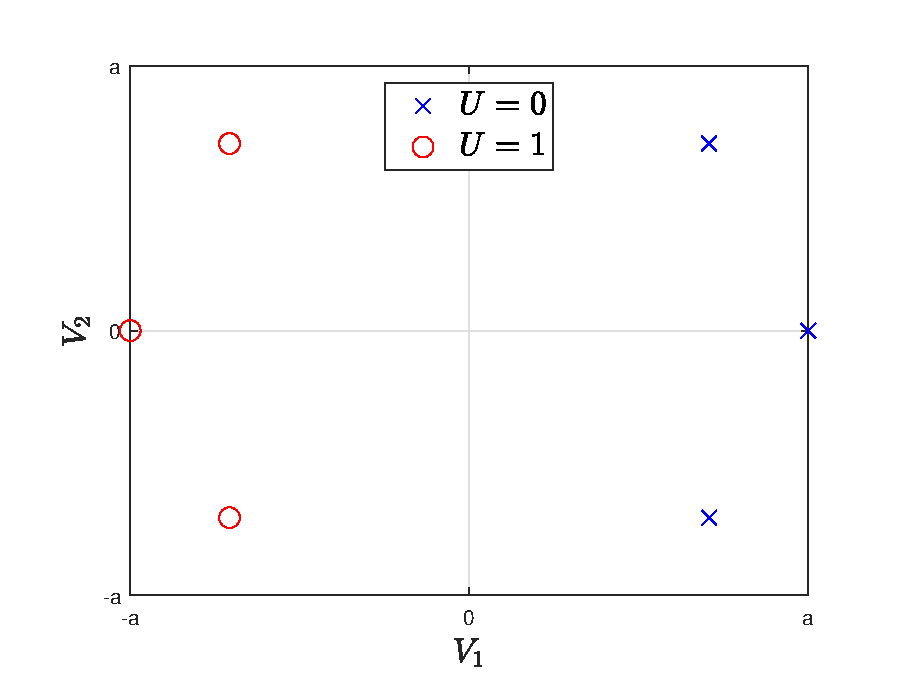
\includegraphics[width=.4\columnwidth]{A-11-P-2.eps}
        \caption{Possible value of $(V_1,V_2)$ if $\bm{Z}=0$.}
        \label{P-2}
    \end{figure}

    According to figure \ref{P-2}, guess that the ML decision rule is
    \begin{align}
        V_1\overset{\hat{U}=0}{\underset{\hat{U}=1}{\gtreqless}}1.
    \end{align}

    Now we prove that the above rule is optimal: The joint pdf of $(V_1,V_2)$ conditional on $U=0$ is
    {\footnotesize
    \begin{align}
        \notag f_{(V_1,V_2)\vert U}((v_1,v_2)\vert U=0)=&\frac{1}{3}\frac{1}{\sqrt{2\pi\sigma^2}}\exp\left[-\frac{\left(v_1-\frac{a}{\sqrt{2}}\right)^2}{2\sigma^2}\right]\frac{1}{\sqrt{2\pi\sigma^2}}\exp\left[-\frac{\left(v_2+\frac{a}{\sqrt{2}}\right)^2}{2\sigma^2}\right]\\
        \notag&+\frac{1}{3}\frac{1}{\sqrt{2\pi\sigma^2}}\exp\left[-\frac{\left(v_1-a\right)^2}{2\sigma^2}\right]\frac{1}{\sqrt{2\pi\sigma^2}}\exp\left[-\frac{v_2^2}{2\sigma^2}\right]\\
        \notag&+\frac{1}{3}\frac{1}{\sqrt{2\pi\sigma^2}}\exp\left[-\frac{\left(v_1-\frac{a}{\sqrt{2}}\right)^2}{2\sigma^2}\right]\frac{1}{\sqrt{2\pi\sigma^2}}\exp\left[-\frac{\left(v_2-\frac{a}{\sqrt{2}}\right)^2}{2\sigma^2}\right]\\
        =&\frac{1}{6\pi\sigma^2}\left\{\exp\left[-\frac{\left(v_1-\frac{a}{\sqrt{2}}\right)^2+\left(v_2+\frac{a}{\sqrt{2}}\right)^2}{2\sigma^2}\right]+\exp\left[-\frac{\left(v_1-a\right)^2+v_2^2}{2\sigma^2}\right]+\exp\left[-\frac{\left(v_1-\frac{a}{\sqrt{2}}\right)^2+\left(v_2-\frac{a}{\sqrt{2}}\right)^2}{2\sigma^2}\right]\right\}.
    \end{align}
    }
    Similarly, the joint pdf of $(V_1,V_2)$ conditional on $U=1$ is
    {\footnotesize
    \begin{align}
        f_{(V_1,V_2)\vert U}((v_1,v_2)\vert U=1)=\frac{1}{6\pi\sigma^2}\left\{\exp\left[-\frac{\left(v_1+\frac{a}{\sqrt{2}}\right)^2+\left(v_2+\frac{a}{\sqrt{2}}\right)^2}{2\sigma^2}\right]+\exp\left[-\frac{\left(v_1+a\right)^2+v_2^2}{2\sigma^2}\right]+\exp\left[-\frac{\left(v_1+\frac{a}{\sqrt{2}}\right)^2+\left(v_2-\frac{a}{\sqrt{2}}\right)^2}{2\sigma^2}\right]\right\}.
    \end{align}
    }
    ML decision rule is
    \begin{align}
        \frac{f_{(V_1,V_2)\vert U}((v_1,v_2)\vert 0)}{f_{(V_1,V_2)\vert U}((v_1,v_2)\vert 1)}\overset{\hat{U}=0}{\underset{\hat{U}=1}{\gtreqless}}&1,\\
        \Longrightarrow\frac{\exp\left[-\frac{\left(v_1-\frac{a}{\sqrt{2}}\right)^2+\left(v_2+\frac{a}{\sqrt{2}}\right)^2}{2\sigma^2}\right]+\exp\left[-\frac{\left(v_1-a\right)^2+v_2^2}{2\sigma^2}\right]+\exp\left[-\frac{\left(v_1-\frac{a}{\sqrt{2}}\right)^2+\left(v_2-\frac{a}{\sqrt{2}}\right)^2}{2\sigma^2}\right]}{\exp\left[-\frac{\left(v_1+\frac{a}{\sqrt{2}}\right)^2+\left(v_2+\frac{a}{\sqrt{2}}\right)^2}{2\sigma^2}\right]+\exp\left[-\frac{\left(v_1+a\right)^2+v_2^2}{2\sigma^2}\right]+\exp\left[-\frac{\left(v_1+\frac{a}{\sqrt{2}}\right)^2+\left(v_2-\frac{a}{\sqrt{2}}\right)^2}{2\sigma^2}\right]}\overset{\hat{U}=0}{\underset{\hat{U}=1}{\gtreqless}}&1,\\
        \Longrightarrow\frac{\exp\left[\frac{\sqrt{2}av_1-\sqrt{2}av_2}{2\sigma^2}\right]+\exp\left[\frac{2av_1}{2\sigma^2}\right]+\exp\left[\frac{\sqrt{2}av_1+\sqrt{2}av_2}{2\sigma^2}\right]}{\exp\left[\frac{-\sqrt{2}av_1-\sqrt{2}av_2}{2\sigma^2}\right]+\exp\left[\frac{-2av_1}{2\sigma^2}\right]+\exp\left[\frac{-\sqrt{2}av_1+\sqrt{2}av_2}{2\sigma^2}\right]}\overset{\hat{U}=0}{\underset{\hat{U}=1}{\gtreqless}}&1,\\
        \Longrightarrow\exp\left[\frac{2\sqrt{2}av_1}{2\sigma^2}\right]\frac{\exp\left[\frac{-\sqrt{2}av_2}{2\sigma^2}\right]+\exp\left[\frac{(2-\sqrt{2})av_1}{2\sigma^2}\right]+\exp\left[\frac{\sqrt{2}av_2}{2\sigma^2}\right]}{\exp\left[\frac{-\sqrt{2}av_2}{2\sigma^2}\right]+\exp\left[\frac{(-2+\sqrt{2})av_1}{2\sigma^2}\right]+\exp\left[\frac{\sqrt{2}av_2}{2\sigma^2}\right]}\overset{\hat{U}=0}{\underset{\hat{U}=1}{\gtreqless}}&1,\\
        \Rightarrow v_1\overset{\hat{U}=0}{\underset{\hat{U}=1}{\gtreqless}}&1.
    \end{align}
\end{sol}
\end{document}